\chapter{Oxygen Reduction in \Nm{}}
\section{Aerobic Reduction of Oxygen}

Modelling oxygen reduction was the simplest both experimentally and mathematically. MC58 cultures were grown in aerobic conditions for around 3 hours, or until the $\mathrm{OD}_{600}$ had reached 0.3-0.9. Cultures were then transferred to the electrode chamber and the oxygen concentration was recorded as the culture respired. Once the culture had become anaerobic it was re-aerated by bubbling air through the culture with a sterile pasteur pipette. This  restored oxygen levels throughout the culture and they began respiring oxygen once more.

In the model, oxygen reduction is described by equation (1) which is the change in oxygen concentration over time. Modelling the reaction also requires equations (4-6) also to describe the flow of electrons into the system and to the terminal reductase. This involved 17 parameters and variables to be estimated.

The experimental dataset shows that oxygen reduction in \textit{Neisseria meningitidis} is a simple linear system with the reductase having a high affinity for oxygen demonstrated by the almost complete lack of non-linearity as oxygen concentration approaches zero. This apparent simple linearity could be modelled with a high degree of accuracy with just 2 parameters in a simple $y=-mx+c$ system. However this does mean that the posterior distributions generated are very wide and therefore allows much greater freedom for the next dataset to explore the parameter space.

The final solved output of the parameter estimation for this dataset can be seen in Figure \ref{fig:o2sim}. The initial parameter set used to start the Monte-Carlo run was one based on some preliminary experimental data (dataset not shown) and priors from literature about sensible concentrations and rate constants for this system. Very little information is readily available in the literature to populate the model.

Given our knowledge of the underlying transport chain and the affinity of \textit{cbb$_{\textrm{3}}$} for oxygen, we expect a linear reduction of oxygen with high affinity over nearly two orders of magnitude. It is however remarkable that we can model this behaviour with so few components in the model, as it requires significant changes in the reduction state of the enzymes to achieve this.

\begin{figure}[ht!]
 \centering
 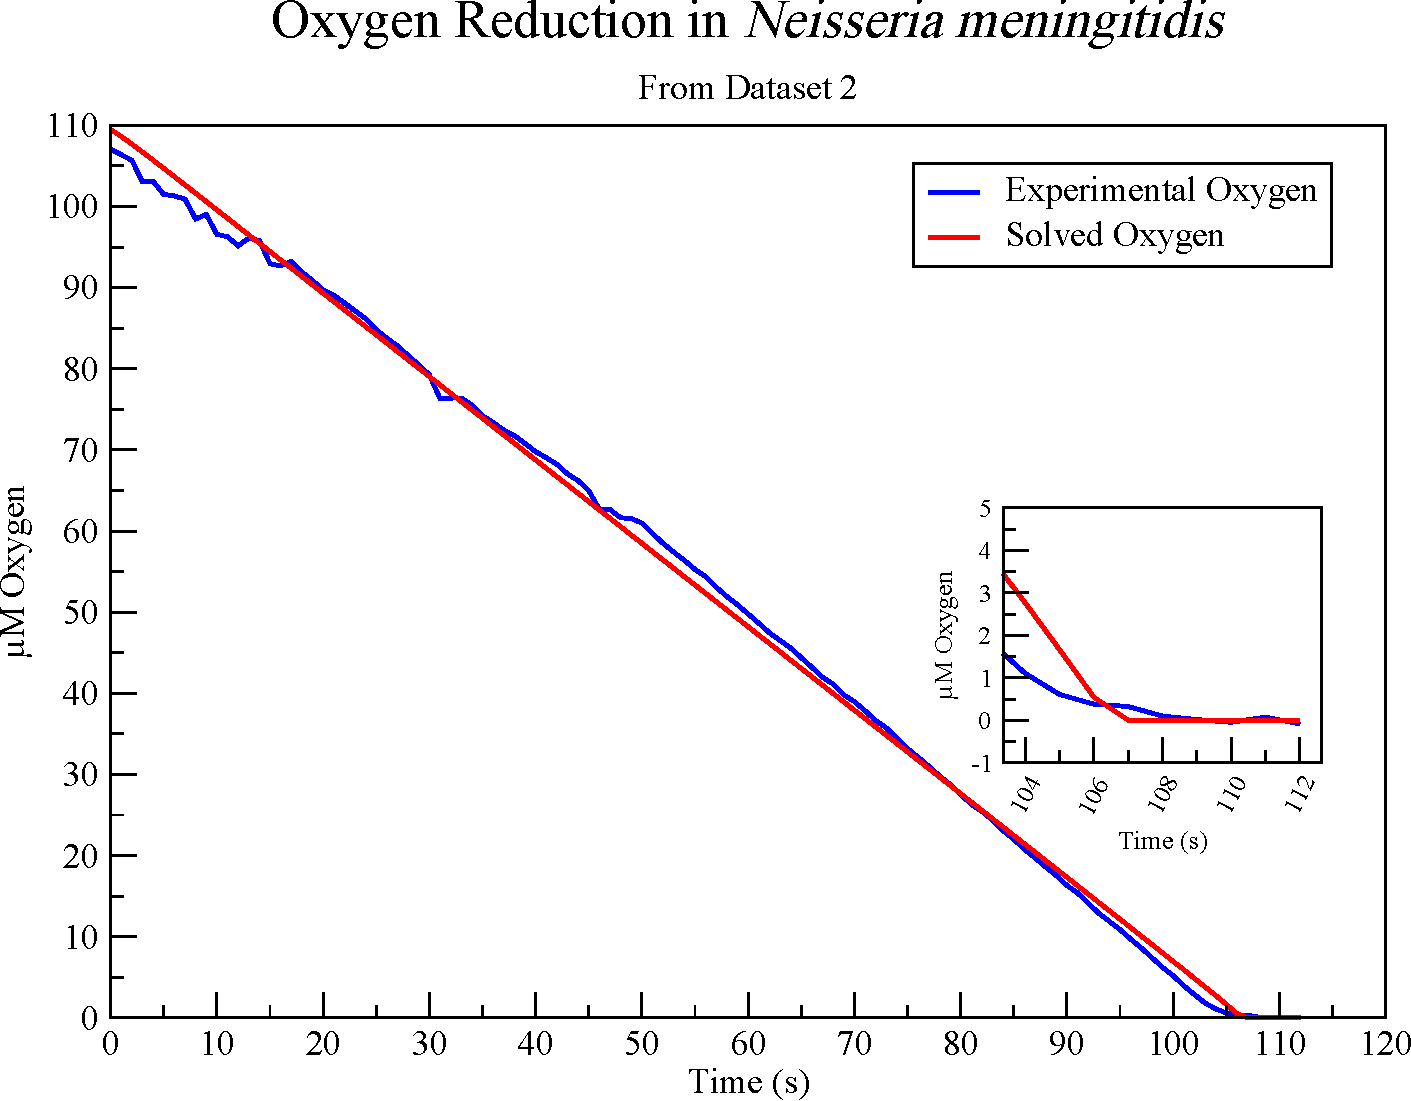
\includegraphics[width=4in]{./05-oxygenreduction/data/o2sim.pdf}
 % o2sim.eps: 0x0 pixel, 300dpi, 0.00x0.00 cm, bb=0 0 794 595
 \caption{{\bf Oxygen Reduction in \textit{Neisseria meningitidis}.} This dataset shows the simple linear reduction of Oxygen in aerobic conditions. The high affinity of $\mathrm{cbb}_3$ for oxygen is evidenced by very little non-linearity at low oxygen concentrations. The solved output is a representative result of the parameter estimation system.}
 \label{fig:o2sim}
\end{figure}

\subsection{Introduction}
\subsection{Results}
\subsection{Discussion}